%%%%%%%%%%%%%%%%%%%%%%%%%%%%%%%%%%%%%%
%%%%%%%%%%%%%%%%%%%%%%%%%%%%%%%%%%%%%%
% Do not edit the TeX file your work
% will be overwritten.  Edit the RnW
% file instead.
%%%%%%%%%%%%%%%%%%%%%%%%%%%%%%%%%%%%%%
%%%%%%%%%%%%%%%%%%%%%%%%%%%%%%%%%%%%%%







We begin the empirical demonstration of our method on two simple generalized
linear models: logistic and Poisson regression.\footnote{Leave-one-out CV may
not be the most appropriate estimator of generalization error in this setting
\citep{rosset:2018:fixed}, but this section is intended only to provide simple
illustrative examples.} In each case, we generate a synthetic dataset $Z =
\{(x_n, y_n) \}_{n=1}^N$ from parameters $(\theta, b)$, where $\theta
\in \mathbb{R}^{100}$ is a vector of regression coefficients and $b \in
\mathbb{R}$ is a bias term. In each experiment, $x_n \in \mathbb{R}^{100}$ is
drawn from a multivariate Gaussian, and $y_n$ is a scalar drawn from a Bernoulli
distribution with the logit link or from a Poisson distribution with the
exponential link.
%

\begin{knitrout}
\definecolor{shadecolor}{rgb}{0.969, 0.969, 0.969}\color{fgcolor}\begin{figure}[!h]

{\centering 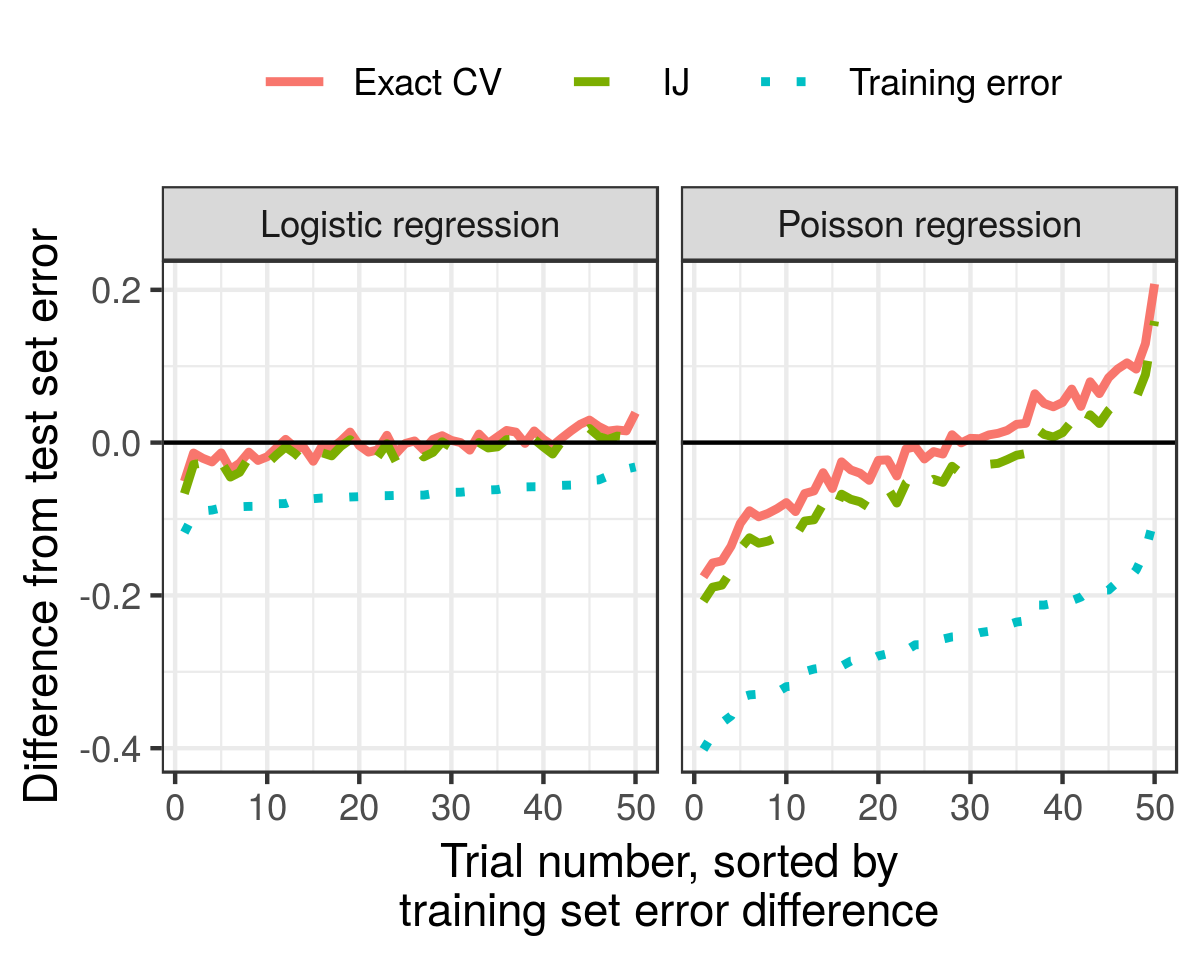
\includegraphics[width=0.98\linewidth,height=0.784\linewidth]{figure/simulated_experiments_accuracy-1} 

}

\caption[Simulated data]{Simulated data: accuracy results.}\label{fig:simulated_experiments_accuracy}
\end{figure}


\end{knitrout}
%
For a ground truth, we generate a large test set with $N=100{,}000$ datapoints
to measure the true generalization error. We show in
\fig{simulated_experiments_accuracy} that, over 50 randomly generated datasets,
our approximation consistently underestimates the actual error predicted by
exact leave-one-out CV; however, the difference is small relative to the
improvements they both make over the error evaluated on the training set.
%

\begin{knitrout}
\definecolor{shadecolor}{rgb}{0.969, 0.969, 0.969}\color{fgcolor}\begin{figure}[!h]

{\centering 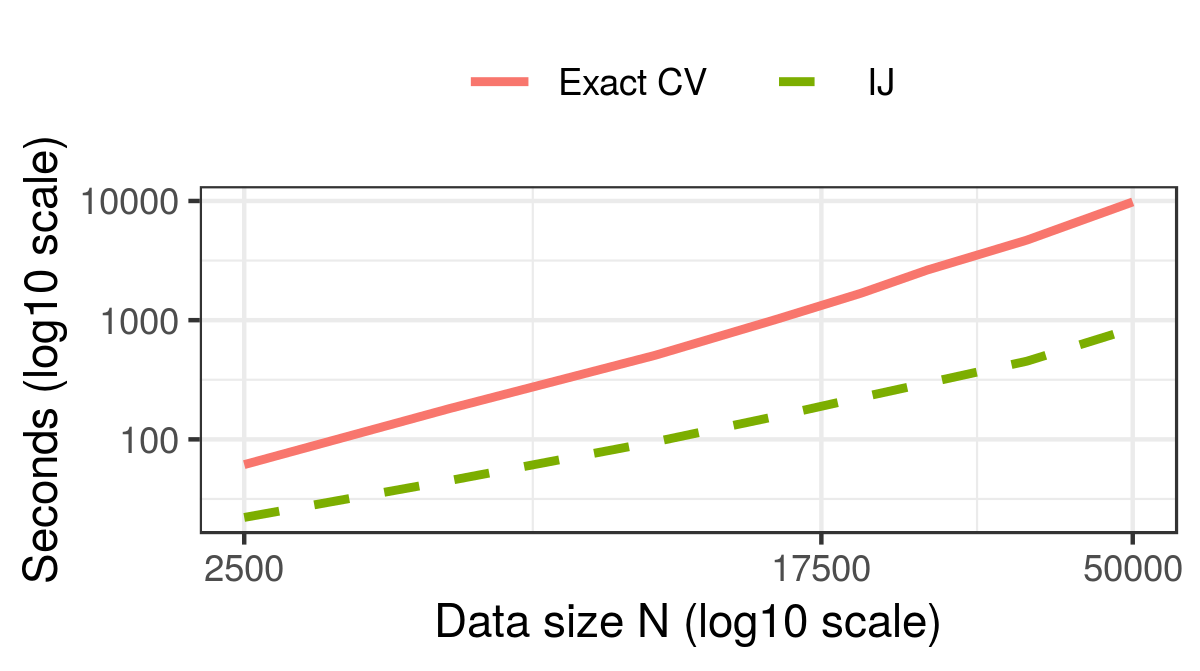
\includegraphics[width=0.98\linewidth,height=0.549\linewidth]{figure/simulated_experiments_timing-1} 

}

\caption[Simulated data]{Simulated data: timing results.}\label{fig:simulated_experiments_timing}
\end{figure}


\end{knitrout}
%
\fig{simulated_experiments_timing} shows the relative timings of our
approximation and exact leave-one-out CV on logistic regression with datasets of
increasing size. The time to run our approximation is roughly an order of
magnitude smaller.
